\documentclass[11pt]{article}
\usepackage{icmlko}
\begin{document}

\title{한 짝의 1.000 이 열한 짝에서 3/11 이 된다}
\author{월드모델 실험실}
\date{노트 431 · 2026년 8월 4일}
\maketitle

\begin{abstract}
노트 429가 $K{=}64$ 를 못 정했다 --- 비게임 앱은 $+0.0075$ 에 되뽑기
$1.000$ 으로 \textbf{확실히} 이겼고 KR 만화는 $-0.0030$ 으로 졌다.
노트 430이 지은 LODO 시험대(도메인 하나씩 빼기)로 \textbf{열한 짝}에
물었다. 사전 등록: \emph{$8$ 이상이면 채택, $3$ 이하면 기각.}

\begin{center}
\begin{tabular}{lr}
\hline
 & $K{=}64 - K{=}32$ \\
\hline
비게임 앱 (노트 429) & $\mathbf{+0.0075}$ \ $[+0.0053, +0.0094]$ \ $\mathbf{1.000}$ \\
\hline
LODO 열한 짝 & \textbf{이긴 도메인 3/11} \\
 & 평균 $-0.0033$ · 중앙값 $-0.0024$ \\
\hline
\end{tabular}
\end{center}

\textbf{기각이다.} 이긴 셋은 게임 $+0.0021$ · 시장팝업 $+0.0015$ · 펀딩
$+0.0010$ 으로 전부 잔돈이고, 진 여덟 중 모바일 $-0.0105$ · 팝업 $-0.0091$ ·
도서 $-0.0069$ 는 그보다 크다. \textbf{노트 396의 ``$K$ 는 포화''가 판에서도
전이에서도 맞다.}

그리고 이 노트의 요점은 $K$ 가 아니다. \textbf{한 짝에서 $1.000$ 이던 것이
열한 짝에서 뒤집혔다.}
\end{abstract}

\section{구간은 행을 재지 도메인을 안 잰다}

되뽑기 구간 $[+0.0053, +0.0094]$ 는 \textbf{그 도메인의 유보 행}을 다시
뽑아 잰 것이다. 앱 1{,}600행을 아무리 다시 뽑아도 나오는 답은
``\emph{이 도메인에서는} 확실히 낫다''이지 ``안 본 도메인에서 낫다''가
아니다. \textbf{도메인을 고르는 불확실성은 그 구간 안에 안 들어 있다.}

이 사이클이 내내 짝 둘로 굴러갔다. 노트 423의 $0.39$, 노트 426의 깊이,
노트 427의 lr --- 전부 짝 둘이다. \textbf{그 중 하나라도 이번 $K$ 처럼
한쪽만 유난한 것이었다면 잘못 채택했을 수 있다.}

\section{규약을 올린다}

노트 426이 ``안 본 도메인 \textbf{둘 이상}에서 같은 부호''를 썼다. 짝이
둘뿐일 때의 임시 조항이었다. 이제 열하나가 있다.

\begin{center}
\textbf{전이 판정은 LODO 열한 짝의 다수결로 한다.}\\
$\ge 8/11$ 채택 · $\le 3/11$ 기각 · 사이는 미결정\\
(한쪽 꼬리 이항 $0.033$ --- 판의 $9/12$ 와 같은 자리)
\end{center}

\section{먼저 내 것부터 다시 봐야 한다}

이번 사이클에 짝 둘로 채택한 것이 셋이다. \textbf{그 중 lr $0.10$ 이
제일 얇다} --- 앱 $+0.0046$ · KR $+0.0121$ 로 둘 다 작다. $K$ 가 앱에서
$+0.0075$ 로 이기고도 열한 짝에서 졌으니, \textbf{$+0.0046$ 은 더 위험하다}.
바로 다음에 건다.

깊이 $12$ 는 앱 $+0.0292$ · KR $+0.0267$ 로 $K$ 보다 네 배 크고 둘이
크기까지 맞았다 --- 덜 위험하지만 역시 열한 짝으로 봐야 한다.

\begin{tabular}{lp{7.0cm}}
\hline
lr $0.10$ & 열한 짝으로 다시. 이번 사이클 채택 중 제일 얇다 \\
깊이 $12$ & 같은 이유, 순서는 그다음 \\
$K$ & 판·전이 둘 다 포화. \textbf{닫는다} \\
\hline
\end{tabular}

\begin{figure}[h]
\centering
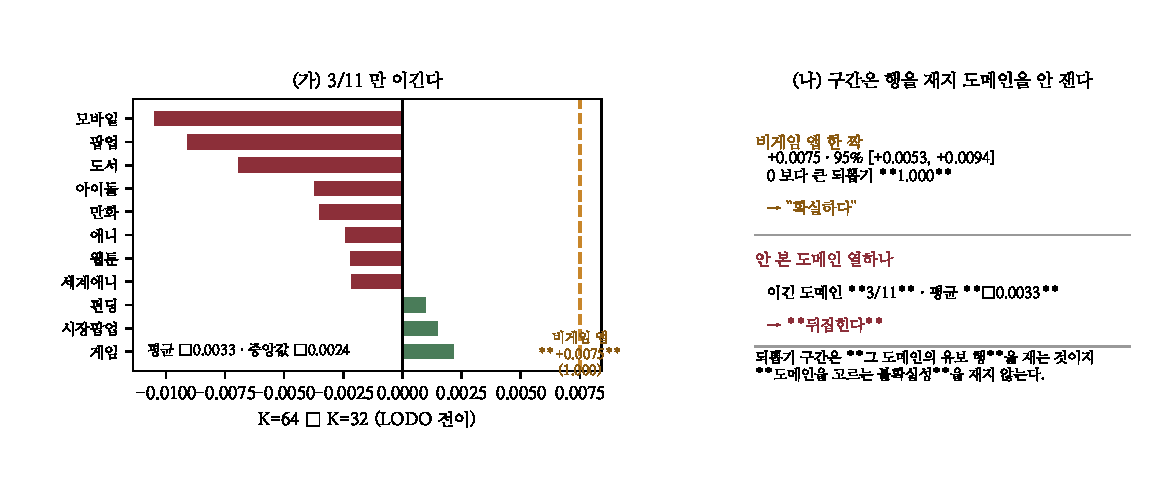
\includegraphics[width=\textwidth]{figs/fig431.pdf}
\caption{(가) 열한 짝 중 셋만 이긴다. 주황 선이 앱 한 짝의 값.
(나) 되뽑기 구간이 무엇을 재고 무엇을 안 재는가.}
\end{figure}

\end{document}
